%%%%%%%%%%%%%%%%%%%%%%%%%%%%%%%%%%%%%%%%%
% APA Assignment Article
% LaTeX Template
% Version 2.0 (February 7, 2023)
%
% This template originates from:
% https://www.LaTeXTemplates.com
%
% Author:
% Vel (vel@latextemplates.com)
%
% License:
% CC BY-NC-SA 4.0 (https://creativecommons.org/licenses/by-nc-sa/4.0/)
%
% NOTE: The bibliography needs to be compiled using the biber engine.
%
%%%%%%%%%%%%%%%%%%%%%%%%%%%%%%%%%%%%%%%%%

%----------------------------------------------------------------------------------------
%	PACKAGES AND OTHER DOCUMENT CONFIGURATIONS
%----------------------------------------------------------------------------------------

\documentclass[
	letterpaper, % Paper size, use either a4paper or letterpaper
	10pt, % Default font size, can also use 11pt or 12pt, although this is not recommended
	unnumberedsections, % Comment to enable section numbering
	twoside, % Two side traditional mode where headers and footers change between odd and even pages, comment this option to make them fixed
]{APAAssignment}

\addbibresource{bibliography.bib} % BibLaTeX bibliography file

\runninghead{MICS CYBER 252, Fall-2024 Hands On Lab Unit 5} % A shortened article title to appear in the running head, leave this command empty for no running head

\footertext{\textit{Hands On Lab Unit 5} (MICS CYBER 252, Fall -2024)} % Text to appear in the footer, leave this command empty for no footer text

\setcounter{page}{1} % The page number of the first page, set this to a higher number if the article is to be part of an issue or larger work

%----------------------------------------------------------------------------------------
%	TITLE SECTION
%----------------------------------------------------------------------------------------

\usepackage[title,toc,titletoc]{appendix}
\usepackage{titlesec}
\usepackage{lscape}
\usepackage{fontawesome}

\title{Hands On Lab Unit 5 \\ MICS-252, Fall 2024} % Article title, use manual lines breaks (\\) to beautify the layout

% Authors are listed in a comma-separated list with superscript numbers indicating affiliations
% \thanks{} is used for any text that should be placed in a footnote on the first page, such as the corresponding author's email, journal acceptance dates, a copyright/license notice, keywords, etc
% Affiliations are output in the \date{} command
\date{UC Berkleley School of Information \\
MICS Course 252 Fall 2024 (Kristy Westphal)
}


\author{
	Prepared by: Karl-Johan Westhoff \\
	email: \href{mailto:kjwesthoff@berkeley.edu}{kjwesthoff@berkeley.edu}
}


% % Full-width abstract
% \renewcommand{\maketitlehookd}{%
% 	\begin{abstract}
% 		\noindent Lorem ipsum dolor sit amet,rta porttitor.
% 	\end{abstract}
% }

%----------------------------------------------------------------------------------------

\setcounter{tocdepth}{5}
\setcounter{secnumdepth}{5}
\usepackage[title]{appendix}

\begin{document}
\onecolumn
\maketitle % Output the title section

%----------------------------------------------------------------------------------------
%	ARTICLE CONTENTS
%----------------------------------------------------------------------------------------


\section{Reverse engineering of executables}\label{log-analysis}
Two files are provided to be analyzed, trying to figure out what they do and if they are malicious.

\section{'file' analysis}
Linux has a simple utility for checking a file' type by its content, see results in Figure \ref{fig:fileAnalysis}
\begin{figure}[!htp] % Single column :figure	
	\centering
	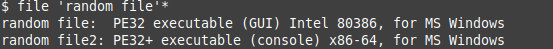
\includegraphics[width=0.7\linewidth]{file_analysis.png}
	\caption{Output from using 'file' in Linux on 'random\_file' and 'random\_file2'}
	\label{fig:fileAnalysis}
\end{figure}

\subsection{'file' Results} The 'PE32' and 'PE32+' indicate the file format is 'Portable Executable' (the '+' indicating version for 64bit memory structure)\cite{PE32Wikipedia}. The PE32 standard includes some headers in the file so the Windows operating can execute the files, either as a stand alone .exe files or as part of other programs or things running on the OS as .dll etc.\footnote{Windows file extensions for PE's include: .acm, .ax, .cpl, .dll, .drv, .efi, .exe, .mui, .ocx, .scr, .sys, .tsp, .mun\cite{PE32Wikipedia}} \\
I.e. the files could contain many functions for something running on a Windows OS. The PE file (ELF files for Linux) contain headers with information of how the program should be laid out in memory on the OS.

\section{'Virus Total'}\label{sec:ViruTotal}
I also threw the files into virus "Virus Total"\cite{VirusTotal} which both subjects the files to signature scanning and provides details and compares it to the contents to other uploads of the file.

\subsection{Virus Total Results} Virus totals findings are listed in Appendix \ref{app:VirusTotal}, Figures \ref{fig:VirusTotalRandomFile} and \ref{fig:VirusTotalRandomFile2}. Results include various file SHA hashings, file formats etc. Furthermore, the is a 'Names' section where previous uploads of the same file listed, apart from other submissions of 'random file' Virus Total\footnote{Looks like others have had the same idea and checked 'random\_files'} finds the following file names:

\begin{itemize}
	\item random\_file = CNMSE.exe, a Canon printer network management software
	\item random\_file2 = alfi\_analyse.exe, not much on google regarding this file, ChatGPT mentions the AFL (American Fuzzing Lop)\cite{AFLWiki}, a tool for software testing by sending unusual inputs to a program. 
\end{itemize}

To confirm if the above findings are correct, next step is trying to reverse engineer the files.

\section{Reverse engineering using Ghidra}
Static reverse engineering includes de-compiling the executables, looking at the code, but not running it. I used 'Ghidra'\cite{Ghidra} for the analysis. 
Ghidra is a software reverse engineering (SRE) tool created and maintained by the NSA\cite{GhidraGithub} made publicly in 2019\footnote{The existence of Ghidra was apparently published already in 2017 as part of a WikiLeaks leak\cite{Vault7leak}} 
Ghidra works as follows:

\begin{enumerate}
	\item The Binary is 'disassembled', the machine code is read from the binary file
	\item Assembly language code is constructed from the machine code and how data is moved around memory. The Assembly language is 'somewhat humanly readable' including comments, readable strings etc. and it is possible to read how data is manipulated by the processor and stored in memory it could look like:  
	\begin{verbatim}
		MOV AL, 61h       ; Load AL with 97 decimal (61 hex)
	\end{verbatim} 
	
	\item Based on the Assembly code, Ghidra constructs C-like code which is more humanly 'interpret-able': \begin{itemize}
		\item It splits parts of the code execution into functions
		\item Puts data into variables.
		\item Provides information on which part of the code is imported from other code (Windows .dll's, C <headers.h> etc.)    
		\item It can even draw a graph on how the various functions are called when the program executes
	\end{itemize}
\end{enumerate}

\subsection{Ghidra Treasure Hunt}
Ghidra chewed away on the files and came up with a de-compilation solution, see example in Figure \ref{fig:Ghidra}

\begin{figure}[!htp] % Single column :figure	
	\centering
	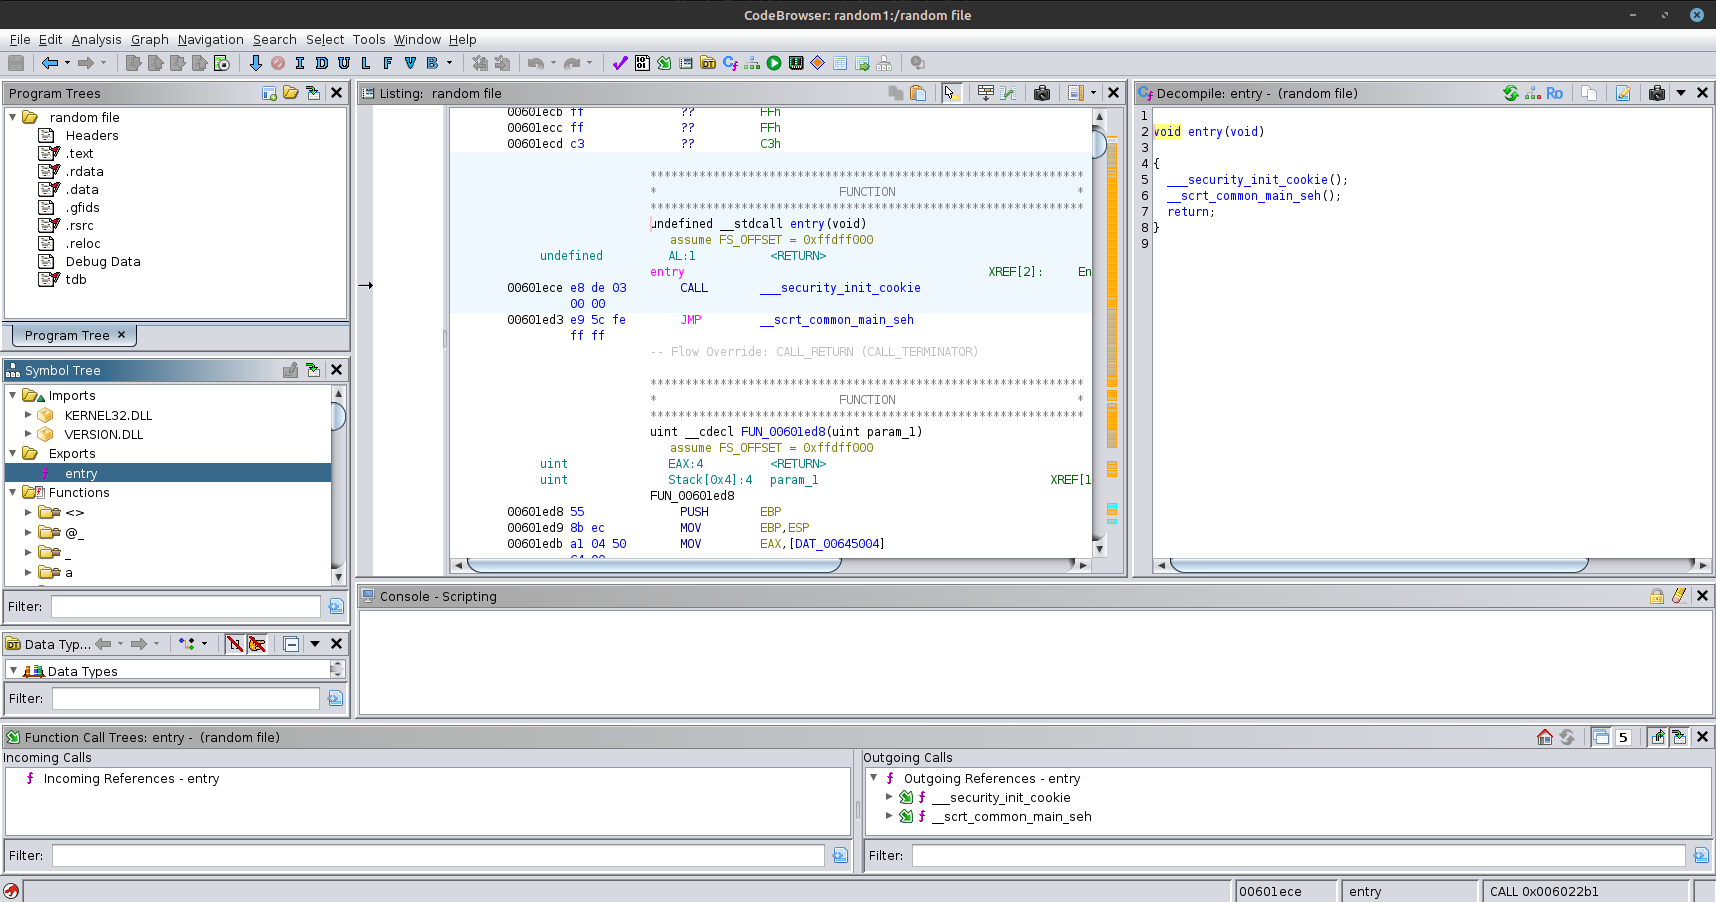
\includegraphics[width=\linewidth]{GhidraRandomFile.png}
	\caption{Ghidra main windows, 'navigation' to the left (see Functions list) Assembly Code in the middle and C code representation to the right, funciton inputs and outputs in the bottom}
	\label{fig:Ghidra}
\end{figure}



To analyze the findings I fist tried to find the entry point function in standard C this is defined as:
\begin{verbatim}
	int main(void);
	int main();
	int main(int argc, char **argv);
	int main(int argc, char *argv[]);
	int main(int argc, char **argv, char **env);
\end{verbatim} 

Looking for functions structured like this was largely un-sucessful (I found multiple functions which fit the schema). Ghidra shows what functions are exposed by the executable for other code to use as an API under "Exports", left side. Here there is an 'entry' function which first checks some security cookie and then runs a function that "does a bunch of stuff" See a graphical tree representation in Appendix \ref{app:GhidraRandomFile}, Figure \ref{fig:GhidraRandomFileTree}. Figuring out what really goes on is subject to a deeper analysis including subject matter experts within the specific type of software (hypothesis from Section \ref{sec:ViruTotal} above being that it is a Canon printer driver). \\
Another way to analyze the bunch of de-compiled code is to look for strings, in this case for 2 purposes:
\begin{enumerate}
	\item Search for the 'Canon' name or 'print*' to confirm that the random file is a Canon printer software
	\item Search for traces of malware. Trojans and malware that connects to a C2 server needs to know where to 'phone home' i.e. they need some hard coded URL's or a way to generate these (if they are trying o obfuscate). An example is the 'SolarWinds' attack, in which C2 url's were obfuscated using a custom hash function to hide from code decompilation\cite{MandiantSW}. So I will look for suspicious URL's and Hash codes. 
\end{enumerate}

\subsection{Ghidra Results, random\_file}
Searching for strings confirmed that the random\_file most likely is a Canon printer software, see Figure \ref{fig:GhidraRandomFileString}. I did not find any suspicious hash codes the files authenticity can be verified against the vendors original file by comparing hash codes.

\begin{figure}[!htp] % Single column :figure	
	\centering
	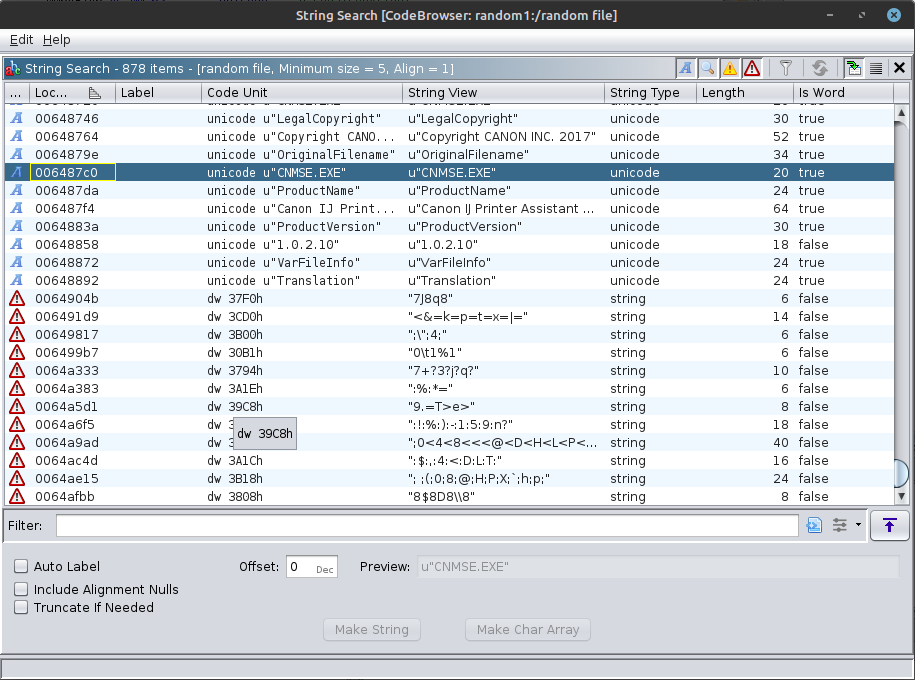
\includegraphics[width=\linewidth]{RandomFileStringSearch.png}
	\caption{String search for strings in the whole de-compiled code, note the vendor name 'Canon' and the CNMSE.EXE string}
	\label{fig:GhidraRandomFileString}
\end{figure}

\subsection{Ghidra Results, random\_file2}
Using the same strategy as above, looking at strings reveal that the file is likely containing a Windows version of the AFL Fuzzing test software. The program flow tree is listed in Appendix \ref{app:GhidraRandomFile2}, Figure \ref{fig:GhidraRandomFile2Tree}. Following the program flow, there are some conditionals that exit the program if conditions are not correct, this is probably reflected in the 'PROGRAM ABORT' strings in Figure \ref{fig:GhidraRandomFileString}.   
\begin{figure}[!htp] % Single column :figure	
	\centering
	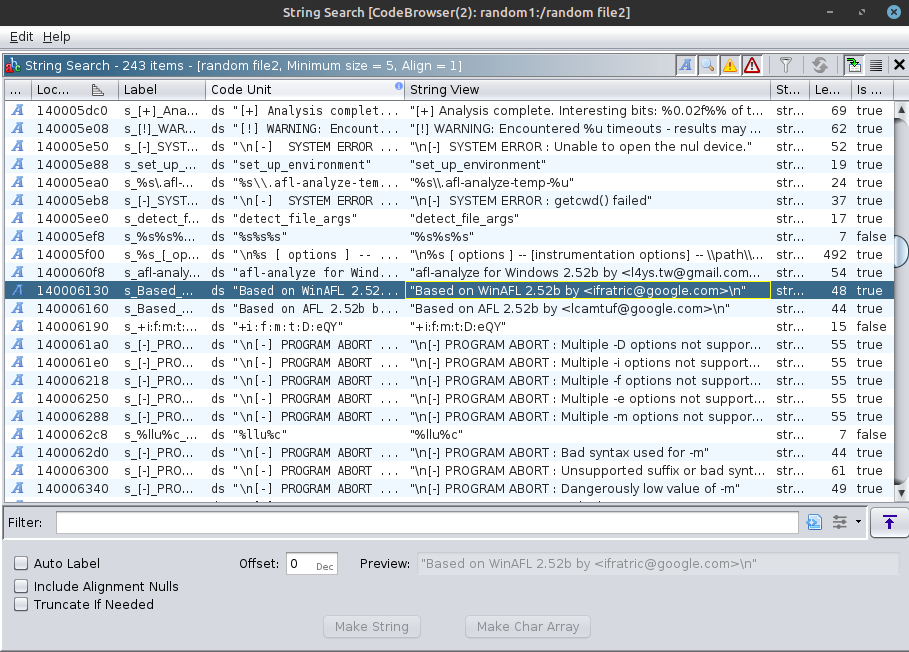
\includegraphics[width=\linewidth]{RandomFile2StringSearch.png}
	\caption{String search for strings in the whole de-compiled code, note the afl\_analyse and WinAFL strings indicating the file is a Windows version of the AFL Fuzzing test software}
	\label{fig:GhidraRandomFile2StringSearch}
\end{figure}

\section{Conclusion}
The files were investigated using various tools: The preinstalled 'file' tool, the online 'Virus Total' and NSA's open source 'Ghidra' tool. The files origins were investigated and identified, further steps would include contacting the original providers of the software for comparison to ensure that no malicious code is hidden in the files (this is of course assuming that there is no malware in the original code either..).  

%----------------------------------------------------------------------------------------
%	 REFERENCES
%----------------------------------------------------------------------------------------
\clearpage
\printbibliography % Output the bibliography

%----------------------------------------------------------------------------------------



%----------------------------------------------------------------------------------------
%	 Appendices
%----------------------------------------------------------------------------------------

\appendix


\clearpage
\chapter{Appendices}
\begin{appendices}

\section{Virus Total Results}\label{app:VirusTotal}
\begin{figure}[!htp] % Single column :figure	
	\centering
	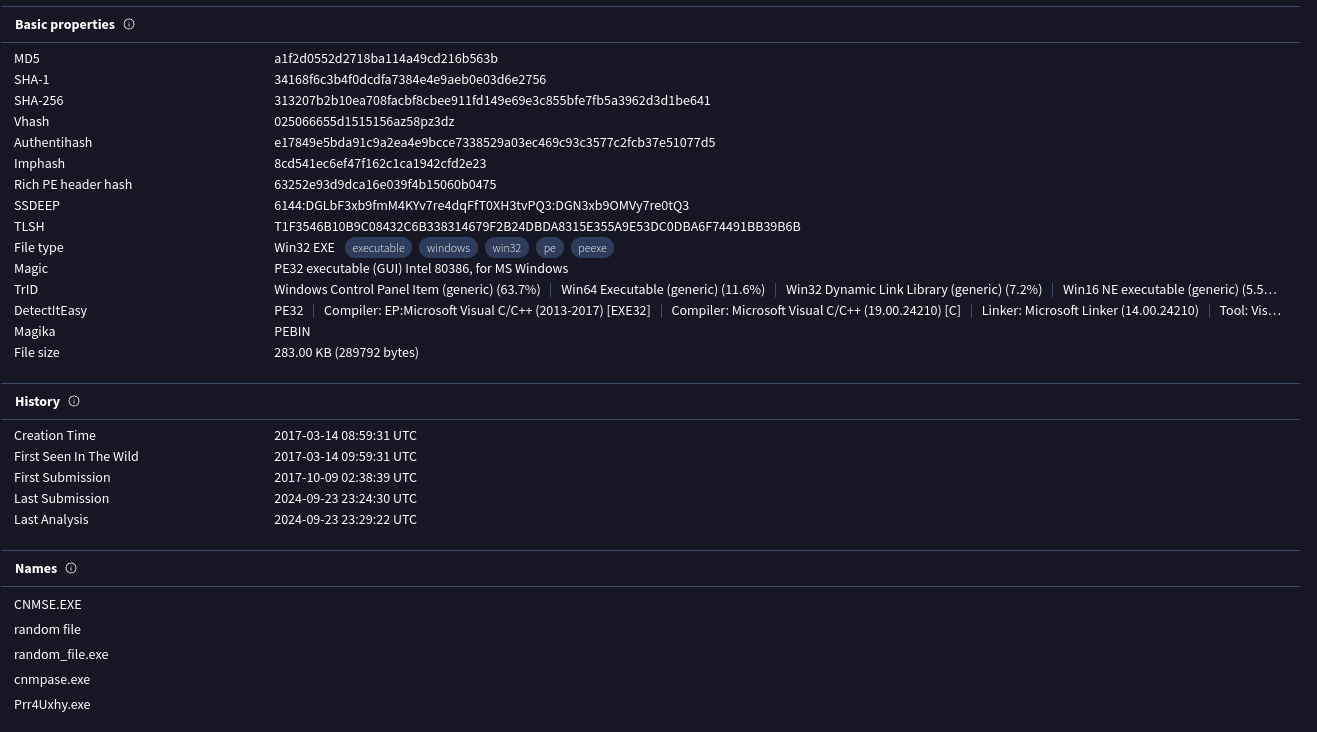
\includegraphics[width=\linewidth]{VirusTotalRandomFile.png}
	\caption{Virus Total details on 'random\_file'}
	\label{fig:VirusTotalRandomFile}
\end{figure}

\begin{figure}[!htp] % Single column :figure	
	\centering
	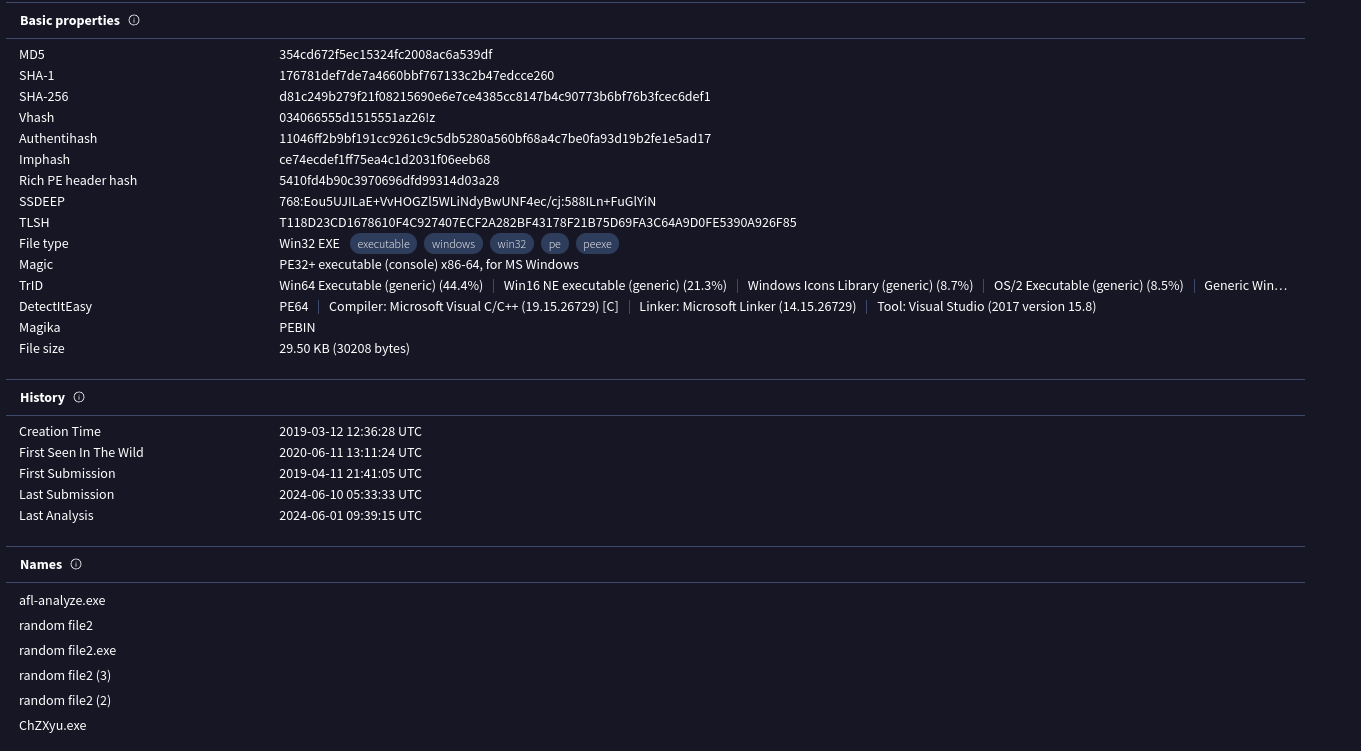
\includegraphics[width=\linewidth]{VirusTotalRandomFile2.png}
	\caption{Virus Total details on 'random\_file2'}
	\label{fig:VirusTotalRandomFile2}
\end{figure}
\clearpage
\section{Ghidra Analyses of 'random\_file'}\label{app:GhidraRandomFile}	
\begin{figure}[!htp] % Single column :figure	
	\centering
	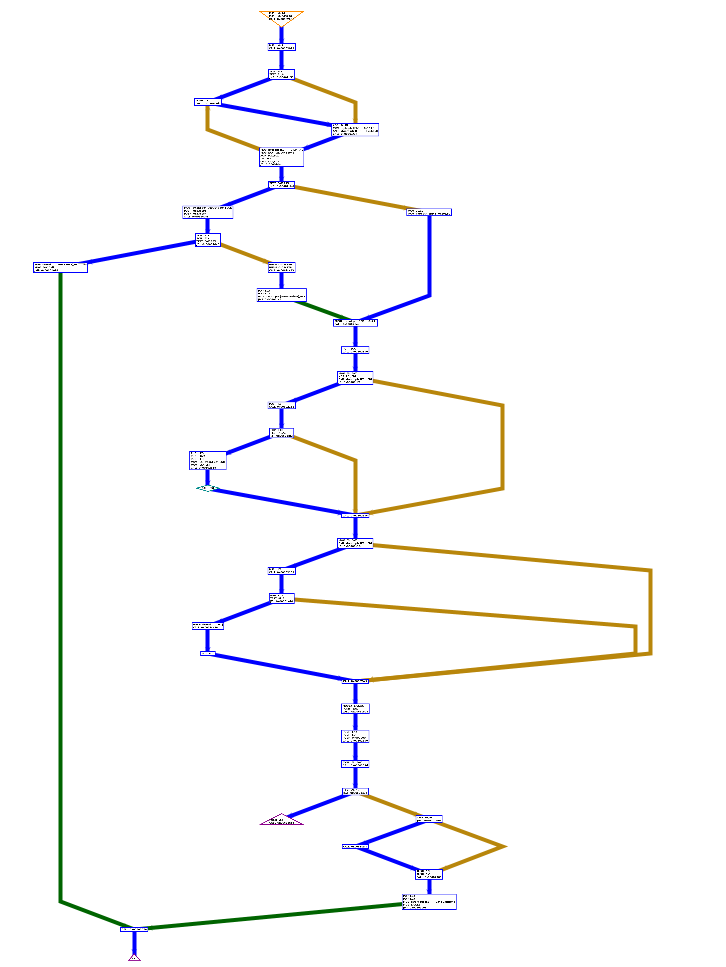
\includegraphics[width=0.8\linewidth]{Random_fileTree.png}
	\caption{'random\_file' scrt\_common\_main\_seh(void) Function as entry point}
	\label{fig:GhidraRandomFileTree}
\end{figure}
\clearpage
\section{Ghidra Analyses of 'random\_file2'}\label{app:GhidraRandomFile2}	
\begin{figure}[!htp] % Single column :figure	
	\centering
	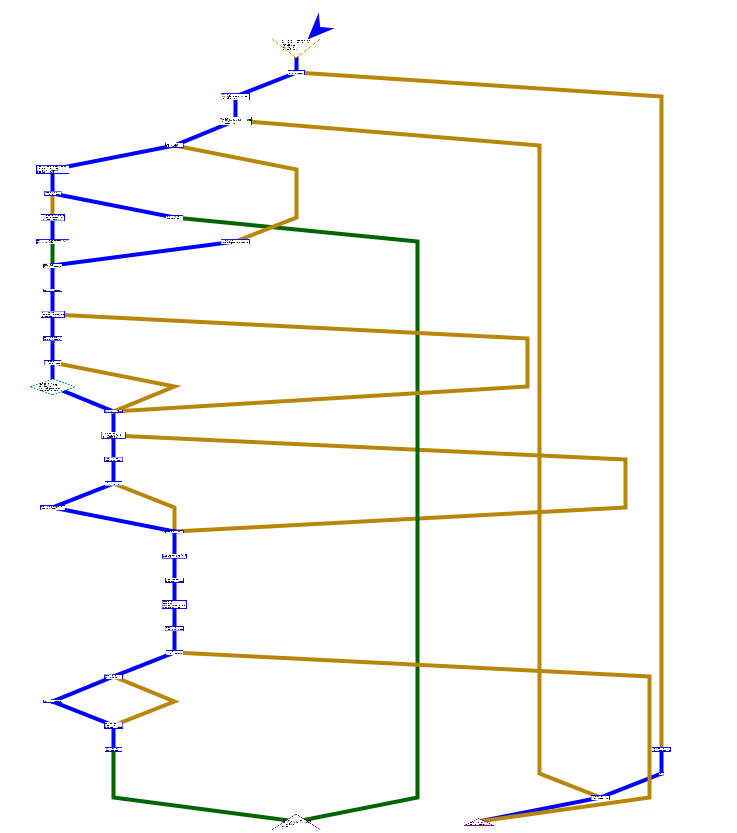
\includegraphics[width=0.8\linewidth]{Random_file2Tree.png}
	\caption{'random\_file2' 'FUN\_140004618(void)' Function as entry point (obviously Ghidra picked the name..)}
	\label{fig:GhidraRandomFile2Tree}
\end{figure}

\begin{figure}[!htp] % Single column :figure	
	\centering
	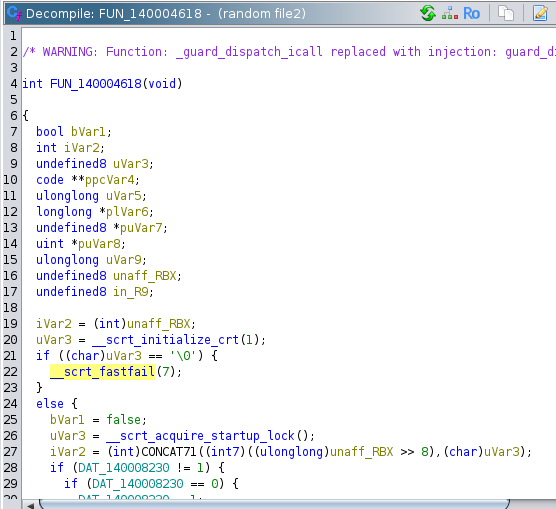
\includegraphics[width=0.8\linewidth]{GhidrafastFail.png}
	\caption{'random\_file2' 'FUN\_140004618(void)' Function a portion of the conditionals execute the 'fastFail' function when they resolve to false}
	\label{fig:GhidraFastFail}
\end{figure}
\end{appendices}
\end{document}
